\chapter{Design}

\section{Overall System Design}

\subsection{Short description of the main parts of the system}

\subsection{System flowcharts showing an overview of the complete system}

\section{User Interface Designs}

\section{Program Structure}

\subsection{Top-down design structure charts}

\subsection{Algorithms in pseudo-code for each data transformation process}

\subsection{Object Diagrams}

\subsection{Class Definitions}

\newpage

\section{Prototyping}

\section{Definition of Data Requirements}

\subsection{Identification of all data input items}

\subsection{Identification of all data output items}

\subsection{Explanation of how data output items are generated}

\subsection{Data Dictionary}

\subsection{Identification of appropriate storage media}

\section{Database Design}

\subsection{Normalisation}

\newpage

\begin{landscape}

\subsubsection{ER Diagrams}

\begin{figure}[H]
    \centerline{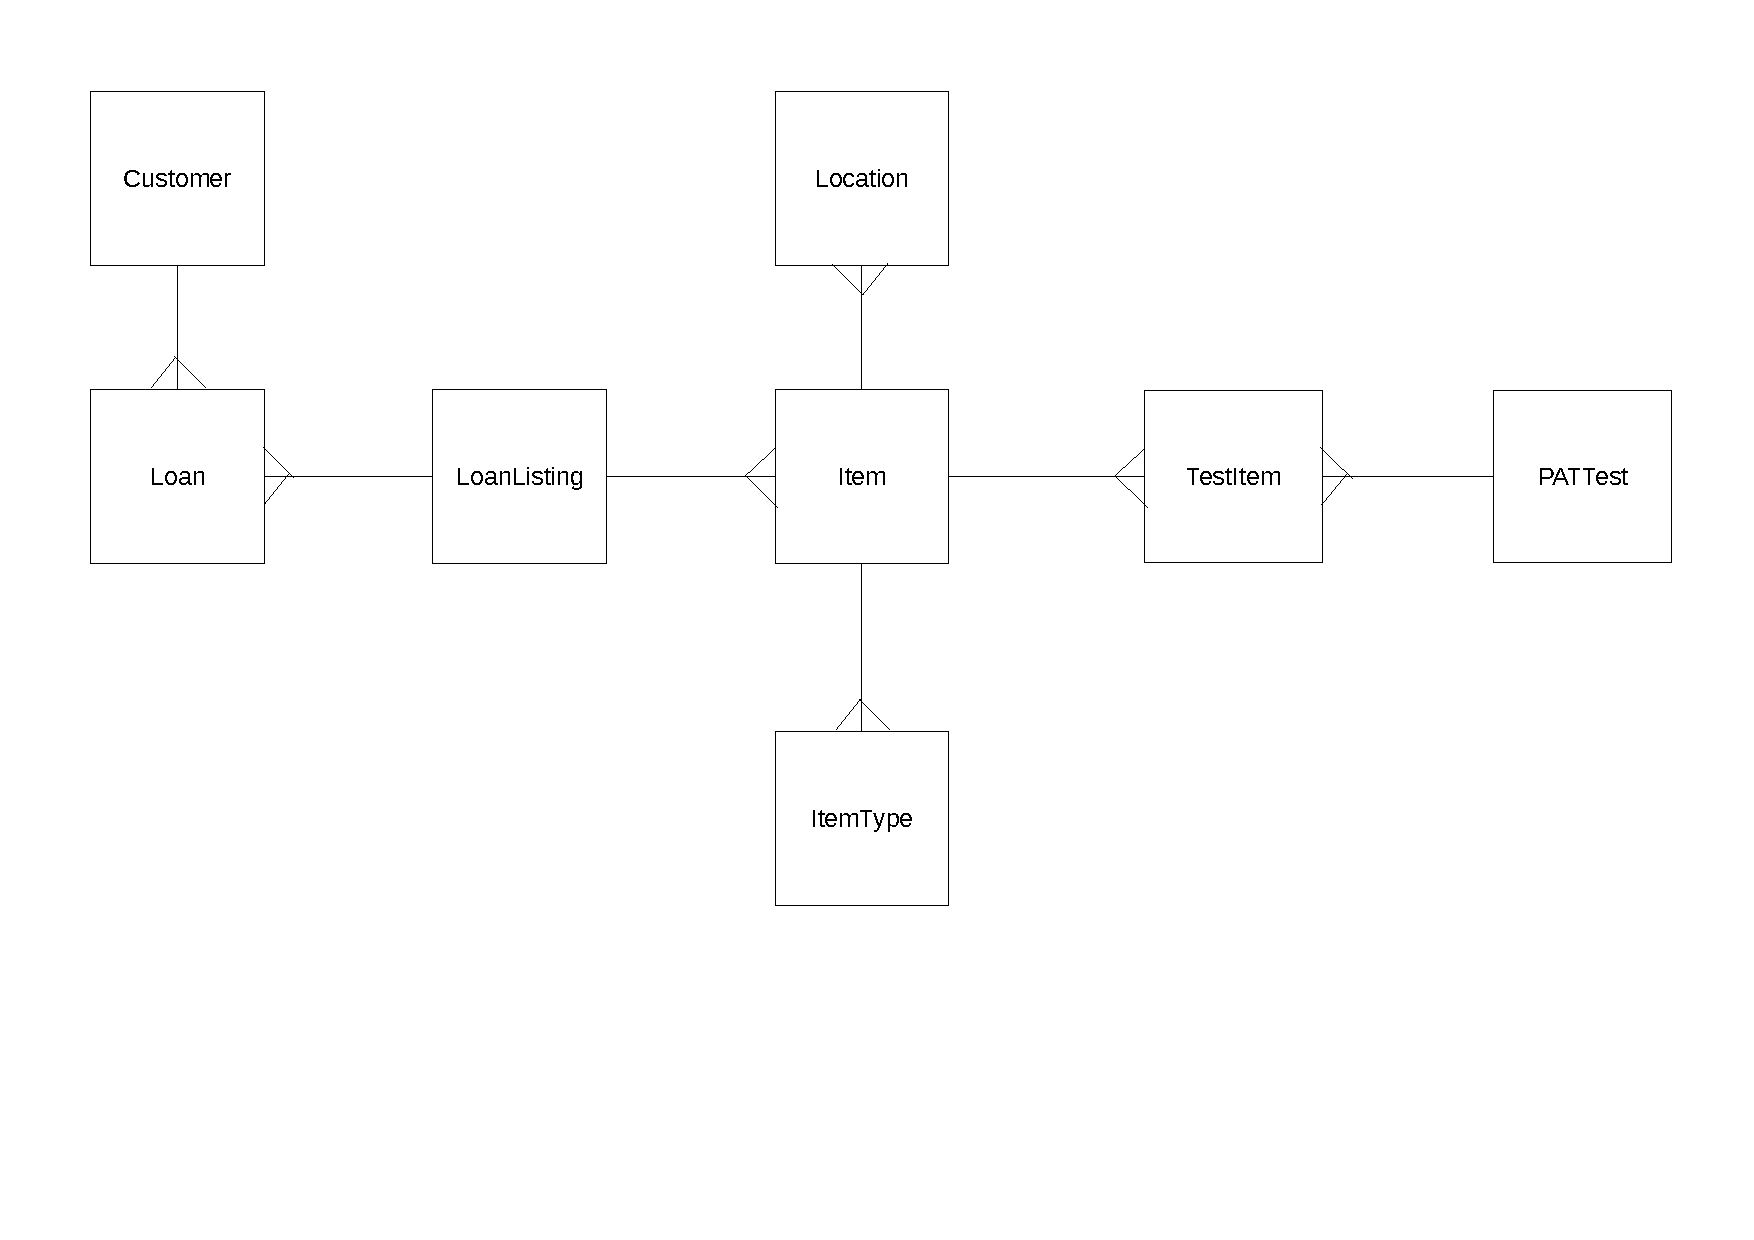
\includegraphics[width=600px]{./Design/Database_Design/Normalisation/ER_Diagrams/ER_Diagram.pdf}}
    \caption{ER Diagrams.} \label{fig:ER Diagrams}
\end{figure}

\end{landscape}

\subsubsection{Entity Descriptions}

\begin{center}
    \begin{tabular}{|c|}
        \hline
        \textbf{Un-Normalised Form(UNF)}\\ \hline
        \underline{ItemID}\\
        ItemName\\
        ItemTypeID\\
        ItemLocationID
        ItemType
        ItemLocation\\ 
        Value\\ 
        ItemQuantity\\ 
        SubTotal\\ 
        OnLoan\\ 
        LoanListingID\\ 
        LoanQuantity\\
        LoanID\\ 
        LoanRate\\ 
        LoanLength\\ 
        LoanCost\\ 
        CustomerID\\ 
        Forename\\ 
        Lastname\\ 
        Company\\ 
        Street\\ 
        Town\\ 
        PostCode\\ 
        MobileNumber\\ 
        LandLine\\ 
        Email\\ 
        PATtestID\\
        TestResult\\ 
        TestDate\\ 
        ItemDescription\\ 
        ItemClass\\ 
        FuseRating\\ 
        TestUsed\\ 
        ProtectiveCondTest\\ 
        InsulationTest\\ 
        Leakage\\ \hline
    \end{tabular}
\end{center}

\newpage

\subsubsection{1NF to 3NF}

\begin{center}
    \begin{tabular}{|c|c|}
        \hline
        \multicolumn{2}{|c|}{\textbf{First-Normalised Form(1NF)}} \\
        \multicolumn{2}{|c|}{ }                                   \\ \hline
        \textbf{Non-Repeating} & \textbf{Repeating}               \\ \hline
        \underline{ItemID}     & \underline{LoanListingID}        \\ 
        ItemName               & \emph{ItemID}                    \\ 
        ItemTypeID             & LoanQuantity                     \\ 
        ItemLocationID         & LoanID                           \\
        Value                  & LoanRate                         \\ 
        ItemQuantity           & LoanLength                       \\ 
        SubTotalValue          & LoanCost                         \\ 
        OnLoan                 & CustomerID                       \\ 
        ItemType               & Forename                         \\ 
        ItemLocation           & Lastname                         \\ 
                               & Company                          \\ 
                               & Street                           \\ 
                               & Town                             \\ 
                               & PostCode                         \\ 
                               & MobileNumber                     \\ 
                               & Landline                         \\ 
                               & Email                            \\ 
                               & PATtestID                        \\ 
                               & TestDate                         \\ 
                               & ItemDescription                  \\ 
                               & ItemClass                        \\ 
                               & FuseRating                       \\ 
                               & TestUsed                         \\ 
                               & ProtectiveCondTest               \\ 
                               & InsulationTest                   \\ 
                               & Leakage                          \\ 
                               & TestResult                       \\ \hline
    \end{tabular}
\end{center}

\newpage

\begin{center}
    \begin{tabular}{|c|c|}
        \hline
        \multicolumn{2}{|c|}{\textbf{Second-Normalised Form(2NF)}} \\
        \multicolumn{2}{|c|}{ }                                    \\ \hline
        \textbf{Non-Repeating}     & \textbf{Repeating}            \\ \hline
        \underline{ItemID}         & \underline{LoanListingID}     \\
        \emph{ItemTypeID}          & \emph{ItemID}                 \\
        \emph{ItemLocationID}      & LoanQuantity                  \\
        ItemName                   &                               \\
        Value                      & LoanID                        \\
        ItemQuantity               & LoanRate                      \\
        SubTotalValue              & LoanLength                    \\          
        OnLoan                     & LoanCost                      \\         
                                   & PATtestID                     \\ 
        \underline{ItemtypeID}     & TestDate                      \\ 
        ItemType                   & ItemDescription               \\ 
                                   & ItemClass                     \\ 
        \underline{ItemLocationID} & FuseRating                    \\ 
        ItemLocation               & TestUsed                      \\ 
                                   & ProtectiveCondTest            \\
                                   & InsulationTest                \\ 
                                   & Leakage                       \\
                                   & TestResult                    \\
                                   & CustomerID                    \\
                                   & Forename                      \\
                                   & Surname                       \\
                                   & Company                       \\
                                   & Street                        \\
                                   & Town                          \\
                                   & PostCode                      \\ 
                                   & MobileNumber                  \\
                                   & Landline                      \\ 
                                   & Email                         \\ \hline                     
    \end{tabular}
\end{center}

\begin{center}
    \begin{tabular}{|c|c|}
        \hline
        \multicolumn{2}{|c|}{\textbf{Third-Normalised Form(2NF)}}  \\
        \multicolumn{2}{|c|}{ }                                    \\ \hline
        \textbf{Non-Repeating}     & \textbf{Repeating}            \\ \hline
        \underline{ItemID}         & \underline{LoanListingID}     \\
        \emph{ItemTypeID}          & \emph{ItemID}                 \\
        \emph{ItemLocationID}      & LoanQuantity                  \\
        ItemName                   &                               \\
        Value                      & \underline{LoanID}            \\
        ItemQuantity               & LoanRate                      \\
        SubTotalValue              & LoanLength                    \\
        OnLoan                     & LoanCost                      \\
                                   &                               \\
        \underline{ItemtypeID}     & \underline{ItemTestID}        \\
        ItemType                   & \emph{ItemID}                 \\
                                   & TestResult                    \\
        \underline{ItemLocationID} &                               \\
        ItemLocation               & \underline{PATtestID}         \\
                                   & TestDate                      \\
                                   & ItemDescription               \\          
                                   & ItemClass                     \\          
                                   & FuseRating                    \\ 
                                   & TestUsed                      \\ 
                                   & ProtectiveCondTest            \\ 
                                   & InsulationTest                \\ 
                                   & Leakage                       \\
                                   &                               \\ 
                                   & \underline{CustomerID}        \\ 
                                   & Forename                      \\
                                   & Surname                       \\ 
                                   & Company                       \\
                                   & Street                        \\
                                   & Town                          \\
                                   & PostCode                      \\ 
                                   & MobileNumber                  \\
                                   & Landline                      \\ 
                                   & Email                         \\ \hline                                                  
    \end{tabular}
\end{center}

\section{Security and Integrity of the System and Data}

\subsection{Security and Integrity of Data}

\subsection{System Security}

\section{Validation}

\section{Testing}

\begin{landscape}
\subsection{Outline Plan}

\begin{center}
    \begin{tabular}{|p{2cm}|p{5cm}|p{5cm}|p{4cm}|}
        \hline
        \textbf{Test Series} & \textbf{Purpose of Test Series} & \textbf{Testing Strategy} & \textbf{Strategy Rationale}\\ \hline
        Example & Example & Example & Example \\ \hline
    \end{tabular}
\end{center}

\subsection{Detailed Plan}

\begin{center}
    \begin{longtable}{|p{1.5cm}|p{2.5cm}|p{2.5cm}|p{2cm}|p{2cm}|p{2cm}|p{2cm}|p{2cm}|}
        \hline
        \textbf{Test Series} & \textbf{Purpose of Test} & \textbf{Test Description} & \textbf{Test Data} & \textbf{Test Data Type (Normal/ Erroneous/ Boundary)} & \textbf{Expected Result} & \textbf{Actual Result} & \textbf{Evidence}\\ \hline
        Example & Example & Example & Example & Example & Example & Example & Example \\ \hline
    \end{longtable}
\end{center}
\end{landscape}
